% =====================================================================
%  Rozdział 4 - wersja robocza do przeredagowania
%  Dane: wyniki/R4 (pomiary 25.10.2026, test uzupełniający SCSV 8.11.2026)
%  Skróty TLS, CTR, CBC, GCM, HMAC, AEAD rozwinąć przy pierwszym użyciu
%  w rozdziale 2 - tu rozwinięte są tylko te, które mogą tam nie wystąpić.
% =====================================================================
\chapter{Analiza ataków na mechanizmy negocjacji sesji i~integralność danych}\label{ch:ataki}

W rozdziale przedstawiono wyniki eksperymentów dotyczących dwóch grup zagrożeń: ingerencji w~negocjację parametrów sesji TLS oraz modyfikacji danych chronionych kryptograficznie bez kontroli integralności. Wszystkie eksperymenty przeprowadzono na stanowisku opisanym w~rozdziale~\ref{ch:srodowisko}, według schematu z~podrozdziału~\ref{sec:metodyka}. Każdy mechanizm badano w~wariancie podatnym i~poprawionym, tym samym skryptem i~w~tych samych warunkach. Przegląd eksperymentów zawiera tabela~\ref{tab:r4-przeglad}. Właściwości mechanizmów, z~których wynikają obserwowane zachowania, omówiono w~rozdziale~\ref{ch:podstawy}; w~tym rozdziale opisano sposób pomiaru i~uzyskane wyniki.

\begin{table}[htbp]
\centering\small
\begin{tabularx}{\textwidth}{@{}c >{\raggedright\arraybackslash}p{3.3cm} L >{\raggedright\arraybackslash}p{2.3cm} >{\raggedright\arraybackslash}p{2.6cm}@{}}
\toprule
\textbf{Podrozdz.} & \textbf{Badany mechanizm} & \textbf{Wariant podatny / poprawiony} & \textbf{Liczba prób} & \textbf{Miara} \\
\midrule
\ref{sec:arp}    & podszycie w~protokole ARP & -- / detekcja inspektorem \kod{arp\_spoof} & 3 ramki & liczba alarmów \\
\ref{sec:tlsneg} & negocjacja wersji TLS & OpenSSL 1.0.2u / nginx 1.27 & 10 + 4 połączenia & wersja, zestaw szyfrów, reakcja na SCSV \\
\ref{sec:ctr}    & ciasteczko sesyjne, szyfr strumieniowy & AES-128-CTR / AES-128-GCM & $2\times200$ + 2 & odsetek przyjętych modyfikacji \\
\ref{sec:cbc}    & ciasteczko sesyjne, szyfr blokowy & AES-128-CBC / AES-128-GCM & $2\times200$ + 1 & odsetek przyjętych modyfikacji \\
\ref{sec:lenext} & podpis żądania API & SHA-256(sekret~$\|$~wiadomość) / HMAC-SHA-256 & $2\times5$ & reakcja serwera \\
\bottomrule
\end{tabularx}
\caption{Przegląd eksperymentów rozdziału~\ref{ch:ataki}}
\label{tab:r4-przeglad}
\end{table}

% ---------------------------------------------------------------------
\section{Wykrywalność podszycia w~protokole ARP}\label{sec:arp}

Ataki analizowane w~dalszej części rozdziału zakładają, że napastnik może obserwować i~modyfikować ruch między klientem a~serwerem, czyli zajmuje pozycję pośrednika (ang. \ang{man-in-the-middle}). W~sieci lokalnej pozycję tę uzyskuje się najczęściej przez wprowadzenie fałszywych powiązań do pamięci podręcznej protokołu odwzorowania adresów (ang. \ang{Address Resolution Protocol}, ARP), który nie uwierzytelnia odpowiedzi (podrozdział~\ref{sec:killchain}). Celem eksperymentu nie było przechwycenie ruchu, lecz sprawdzenie, czy taka próba jest widoczna dla czujnika systemu detekcji włamań.

\subsection*{Przebieg pomiaru}

Czujnik zapisywał ruch w~sieci \kod{labnet} programem tcpdump. Z~maszyny klienta wysłano w~odstępach około 1~s trzy ramki odpowiedzi ARP, w~których adres IP serwera (10.10.10.30) powiązano z~adresem sprzętowym (ang. \ang{Media Access Control}, MAC) karty sieciowej klienta. Powiązanie to jest sprzeczne ze wzorcem wpisanym do konfiguracji inspektora \kod{arp\_spoof} systemu Snort (tabela~\ref{tab:arp-wzorzec}). Zapisany ruch przeanalizowano następnie offline, uruchamiając Snort z~konfiguracją laboratorium.

\begin{table}[htbp]
\centering\small
\begin{tabular}{@{}lll@{}}
\toprule
\textbf{Maszyna} & \textbf{Adres IP} & \textbf{Adres MAC (wzorzec)} \\
\midrule
\kod{client} & 10.10.10.20 & \kod{08:00:27:3b:7f:6d} \\
\kod{server} & 10.10.10.30 & \kod{08:00:27:f7:36:74} \\
\bottomrule
\end{tabular}
\caption{Wzorcowe powiązania adresów wpisane do konfiguracji inspektora \kod{arp\_spoof}}
\label{tab:arp-wzorzec}
\end{table}

\subsection*{Wyniki}

Zapis ruchu z~czasu eksperymentu zawiera sześć ramek ARP (tabela~\ref{tab:arp-ramki}). Pierwsze trzy to ogłoszenia (ang. \ang{gratuitous ARP}), w~których klient rozgłasza poprawne powiązanie własnego adresu. Kolejne trzy to badane odpowiedzi, przypisujące adres serwera adresowi sprzętowemu klienta. Zestawienie ramek odczytano bezpośrednio z~pliku \kod{arp41.pcap}, a~alarmy z~wyjścia programu Snort (rysunek~\ref{rys:snort-arp}).

\begin{table}[htbp]
\centering\small
\begin{tabularx}{\textwidth}{@{}c r l l l L@{}}
\toprule
\textbf{Nr} & \textbf{Czas [s]} & \textbf{Operacja} & \textbf{Nadawca: IP} & \textbf{Nadawca: MAC} & \textbf{Alarmy} \\
\midrule
1 & 0,000 & zapytanie (ogłoszenie) & 10.10.10.20 & \kod{08:00:27:3b:7f:6d} & brak \\
2 & 0,100 & zapytanie (ogłoszenie) & 10.10.10.20 & \kod{08:00:27:3b:7f:6d} & brak \\
3 & 0,400 & zapytanie (ogłoszenie) & 10.10.10.20 & \kod{08:00:27:3b:7f:6d} & brak \\
4 & 0,825 & odpowiedź & \textbf{10.10.10.30} & \kod{08:00:27:3b:7f:6d} & 112:3, 112:4 \\
5 & 1,827 & odpowiedź & \textbf{10.10.10.30} & \kod{08:00:27:3b:7f:6d} & 112:3, 112:4 \\
6 & 2,828 & odpowiedź & \textbf{10.10.10.30} & \kod{08:00:27:3b:7f:6d} & 112:3, 112:4 \\
\bottomrule
\end{tabularx}
\caption{Ramki ARP zarejestrowane przez czujnik w~czasie eksperymentu (czas liczony od pierwszej ramki)}
\label{tab:arp-ramki}
\end{table}

\begin{figure}[htbp]
\centering
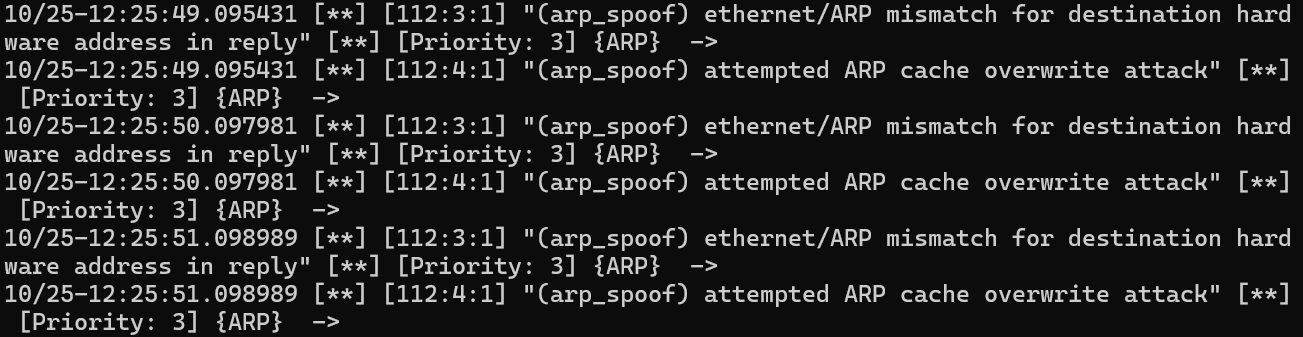
\includegraphics[width=\textwidth]{rysunki/r4-snort-arp.png}
\caption{Alarmy inspektora \kod{arp\_spoof} dla trzech odpowiedzi ARP sprzecznych ze wzorcem}
\label{rys:snort-arp}
\end{figure}

Każda z~trzech odpowiedzi wywołała dwa alarmy o~priorytecie~3, opatrzone tym samym znacznikiem czasu co ramka (łącznie sześć alarmów). Ogłoszenia klienta dotyczące jego własnego, poprawnego powiązania nie wywołały żadnego alarmu. Znaczenie obu typów alarmów podano w~tabeli~\ref{tab:arp-alarmy}.

\begin{table}[htbp]
\centering\small
\begin{tabularx}{\textwidth}{@{}l >{\raggedright\arraybackslash}p{5.1cm} L c@{}}
\toprule
\textbf{Identyfikator} & \textbf{Komunikat} & \textbf{Przyczyna w~badanej ramce} & \textbf{Liczba} \\
\midrule
112:3 & \ang{ethernet/ARP mismatch for destination hardware address in reply} & adres docelowy w~nagłówku Ethernet (rozgłoszeniowy) różni się od adresu docelowego w~treści odpowiedzi ARP & 3 \\
112:4 & \ang{attempted ARP cache overwrite attack} & odpowiedź wiąże adres IP serwera z~innym adresem MAC niż wzorcowy & 3 \\
\bottomrule
\end{tabularx}
\caption{Alarmy zgłoszone przez inspektor \kod{arp\_spoof}}
\label{tab:arp-alarmy}
\end{table}

Wynik potwierdza, że próba podszycia się pod serwer w~warstwie łącza danych pozostawia ślad wykrywalny dla czujnika: wykryto 3 z~3~badanych ramek. Skuteczność ta ma jednak dwa warunki. Po pierwsze, alarm 112:4, który bezpośrednio wskazuje na próbę nadpisania powiązania, może powstać wyłącznie dla adresów wpisanych do wzorca -- inspektor nie chroni maszyn, których powiązań nie skonfigurowano. Po drugie, alarmy w~formacie \kod{alert\_fast} nie zawierają adresów, więc ustalenie, którego powiązania dotyczyła próba, wymaga sięgnięcia do zapisu ruchu. Zachowanie inspektora wobec zwykłego ruchu sieciowego, w~tym liczbę fałszywych alarmów, oceniono w~podrozdziale~\ref{sec:ids}.

% ---------------------------------------------------------------------
\section{Negocjacja wersji protokołu TLS i~sygnalizacja obniżenia wersji}\label{sec:tlsneg}

Pośrednik w~komunikacji może próbować skłonić strony do zestawienia sesji w~najsłabszej wspólnie obsługiwanej wersji protokołu (ang. \ang{downgrade}). O~tym, czy taka próba może się powieść, decyduje przede wszystkim zbiór wersji akceptowanych przez serwer. Badanie obejmowało dwa serwery opisane w~podrozdziale~\ref{sec:serwer}: serwer w~konfiguracji przestarzałej (OpenSSL 1.0.2u, port 4433) i~serwer w~konfiguracji utwardzonej (nginx 1.27, port 443).

\subsection*{Przebieg pomiaru}

Skrypt \kod{r4-skan-tls.sh} uruchomiony na maszynie klienta próbował zestawić z~każdym serwerem połączenie w~każdej z~wersji od SSLv3 do TLS~1.3, za każdym razem dopuszczając tylko jedną wersję. Do wersji TLS~1.2 i~1.3 użyto systemowej biblioteki OpenSSL 3.0.13, a~do wersji starszych -- biblioteki OpenSSL 1.0.2u, ponieważ biblioteka współczesna nie pozwala ich już użyć. Połączenie uznawano za zaakceptowane, jeżeli strony wynegocjowały zestaw szyfrów; w~przeciwnym razie -- za odrzucone. Łącznie wykonano 10~prób połączenia.

\subsection*{Wyniki}

Wyniki zestawiono w~tabeli~\ref{tab:tls-wersje}, a~wyjście skryptu przedstawiono na rysunku~\ref{rys:skan-tls}. Serwer przestarzały zaakceptował cztery z~pięciu wersji, w~tym SSLv3. Dla wersji SSLv3, TLS~1.0 i~TLS~1.1 wynegocjował zestaw \kod{ECDHE-RSA-AES256-SHA}, czyli szyfr w~trybie CBC z~kodem uwierzytelniającym HMAC-SHA1, ponieważ zestawy z~uwierzytelnionym szyfrowaniem (ang. \ang{Authenticated Encryption with Associated Data}, AEAD) są dostępne dopiero od TLS~1.2. Odrzucenie wersji TLS~1.3 nie jest wynikiem utwardzenia, lecz braku jej implementacji w~bibliotece OpenSSL 1.0.2u. Serwer utwardzony zaakceptował wyłącznie TLS~1.2 i~1.3, w~obu przypadkach z~zestawem AEAD, co odpowiada zaleceniu wycofania wersji TLS~1.0 i~1.1 zawartemu w~RFC~8996~\cite{rfc8996}.

\begin{table}[htbp]
\centering\small
\begin{tabularx}{\textwidth}{@{}l L L@{}}
\toprule
\textbf{Wersja} & \textbf{Serwer utwardzony (nginx, :443)} & \textbf{Serwer przestarzały (OpenSSL 1.0.2u, :4433)} \\
\midrule
SSLv3   & odrzucona & zaakceptowana, \kod{ECDHE-RSA-AES256-SHA} \\
TLS~1.0 & odrzucona & zaakceptowana, \kod{ECDHE-RSA-AES256-SHA} \\
TLS~1.1 & odrzucona & zaakceptowana, \kod{ECDHE-RSA-AES256-SHA} \\
TLS~1.2 & zaakceptowana, \kod{ECDHE-RSA-AES128-GCM-SHA256} & zaakceptowana, \kod{ECDHE-RSA-AES256-GCM-SHA384} \\
TLS~1.3 & zaakceptowana, \kod{TLS\_AES\_256\_GCM\_SHA384} & odrzucona \\
\midrule
\textbf{Razem} & \textbf{2 z~5} & \textbf{4 z~5} \\
\bottomrule
\end{tabularx}
\caption{Wersje protokołu akceptowane przez serwery i~wynegocjowane zestawy szyfrów}
\label{tab:tls-wersje}
\end{table}

\begin{figure}[htbp]
\centering
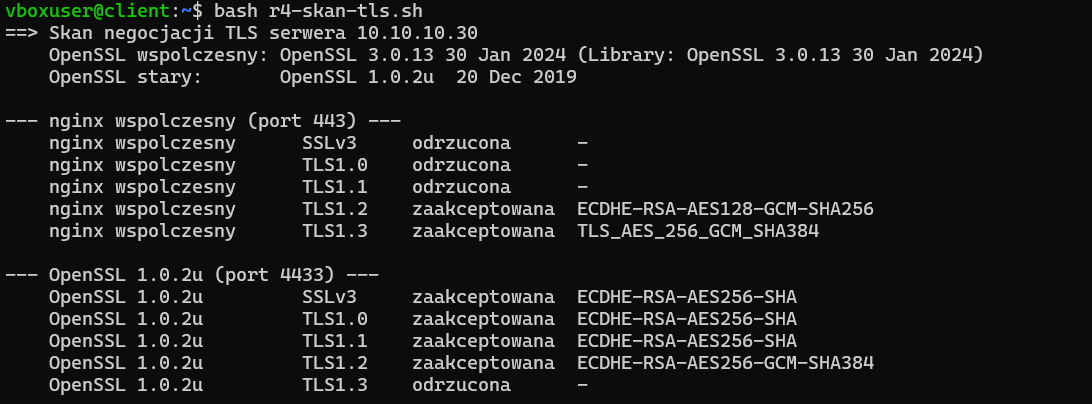
\includegraphics[width=\textwidth]{rysunki/r4-skan-tls.png}
\caption{Wynik skanu wersji protokołu wykonanego skryptem \kod{r4-skan-tls.sh}}
\label{rys:skan-tls}
\end{figure}

Drugą linią obrony przed obniżeniem wersji jest sygnalizacja \kod{TLS\_FALLBACK\_SCSV} (ang. \ang{Signaling Cipher Suite Value}, SCSV), opisana w~RFC~7507~\cite{rfc7507}. Klient, który ponawia nieudane połączenie w~niższej wersji, dołącza do oferty specjalną wartość. Serwer odrzuca takie połączenie alertem \ang{inappropriate\_fallback} (numer 86), ale tylko wtedy, gdy sam obsługuje wersję wyższą niż zaoferowana. W~ramach skanu sprawdzono reakcję obu serwerów na ofertę TLS~1.2 z~sygnałem SCSV. Serwer utwardzony połączenie odrzucił, ponieważ obsługuje TLS~1.3. Serwer przestarzały połączenie przyjął, co jest jednak zgodne ze standardem: TLS~1.2 jest jego wersją najwyższą, a~zatem test ten nie rozstrzygał, czy serwer obsługuje mechanizm SCSV.

Dlatego wykonano test uzupełniający (skrypt \kod{r4-scsv.sh}), w~którym serwerowi przestarzałemu zaoferowano wersje niższe od jego maksymalnej -- z~sygnałem SCSV i~bez niego. Wyniki czterech przypadków zawiera tabela~\ref{tab:scsv}, a~wyjście skryptu rysunek~\ref{rys:scsv}.

\begin{table}[htbp]
\centering\small
\begin{tabularx}{\textwidth}{@{}c l l c L@{}}
\toprule
\textbf{Nr} & \textbf{Serwer} & \textbf{Oferowana wersja} & \textbf{SCSV} & \textbf{Wynik} \\
\midrule
1 & przestarzały (:4433) & TLS~1.1 & tak & odrzucone, alert 86 \\
2 & przestarzały (:4433) & TLS~1.0 & tak & odrzucone, alert 86 \\
3 & przestarzały (:4433) & TLS~1.1 & nie & zestawione: TLS~1.1, \kod{ECDHE-RSA-AES256-SHA} \\
4 & utwardzony (:443)    & TLS~1.2 & tak & odrzucone, alert 86 \\
\bottomrule
\end{tabularx}
\caption{Reakcja serwerów na sygnał obniżenia wersji (test uzupełniający)}
\label{tab:scsv}
\end{table}

\begin{figure}[htbp]
\centering
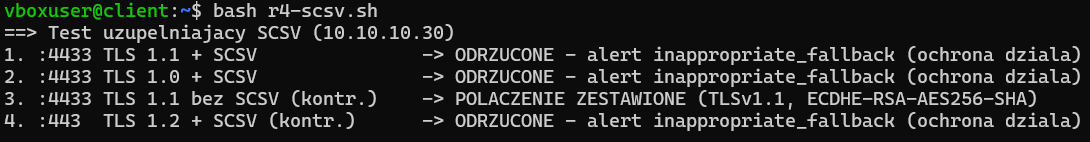
\includegraphics[width=\textwidth]{rysunki/r4-scsv.png}
\caption{Wynik testu uzupełniającego reakcji na sygnał \kod{TLS\_FALLBACK\_SCSV}}
\label{rys:scsv}
\end{figure}

Serwer przestarzały obsługuje mechanizm SCSV poprawnie: odrzucił obie oferty niższych wersji opatrzone sygnałem (przypadki 1 i~2). Ta sama oferta TLS~1.1 bez sygnału (przypadek~3) została jednak przyjęta. Mechanizm SCSV chroni więc wyłącznie klientów, którzy sami sygnalizują obniżenie wersji; klient przestarzały albo skonfigurowany do używania starszej wersji zostanie obsłużony bez zastrzeżeń. Rzeczywistą słabością serwera przestarzałego nie jest zatem brak mechanizmu sygnalizacji, lecz akceptowanie wersji SSLv3, TLS~1.0 i~TLS~1.1. Skuteczną ochroną okazało się dopiero wyłączenie tych wersji po stronie serwera, jak w~konfiguracji utwardzonej. Ruch z~opisanych połączeń zarejestrowany przez czujnik wykorzystano w~podrozdziale~\ref{sec:ids} do oceny reguł wykrywających przestarzałe parametry sesji.

% ---------------------------------------------------------------------
\section{Modyfikacja ciasteczka szyfrowanego w~trybie CTR}\label{sec:ctr}

Eksperymenty z~podrozdziałów~\ref{sec:ctr} i~\ref{sec:cbc} dotyczą ciasteczka sesyjnego aplikacji testowej, które w~zaszyfrowanej postaci przechowuje tekst \kod{user=student;admin=0;uid=1001} (29~bajtów). Pole \kod{admin} decyduje o~dostępie do funkcji administracyjnych. Budowę tokenu w~poszczególnych wariantach przedstawiono w~tabeli~\ref{tab:tokeny}.

\begin{table}[htbp]
\centering\small
\begin{tabularx}{\textwidth}{@{}l L c@{}}
\toprule
\textbf{Wariant} & \textbf{Budowa tokenu (przed kodowaniem Base64)} & \textbf{Długość} \\
\midrule
AES-128-CTR & licznik początkowy (8~B) + kryptogram (29~B) & 37~B \\
AES-128-CBC & wektor inicjujący (16~B) + kryptogram (2 bloki po 16~B, w~tym 3~B dopełnienia) & 48~B \\
AES-128-GCM & wartość jednorazowa (12~B) + kryptogram (29~B) + znacznik uwierzytelniający (16~B) & 57~B \\
\bottomrule
\end{tabularx}
\caption{Budowa tokenu ciasteczka sesyjnego w~badanych wariantach}
\label{tab:tokeny}
\end{table}

\subsection*{Przebieg pomiaru}

Pomiar wykonał skrypt \kod{r4-pomiar-integralnosci.py} uruchomiony na maszynie klienta. Skrypt logował się do aplikacji jako użytkownik \kod{student}, otrzymywał ciasteczko, a~następnie wykonywał dwa rodzaje prób:
\begin{itemize}
  \item \textbf{seria losowa} -- 200~prób dla każdego wariantu; w~każdej próbie zmieniano jeden bajt tokenu na losowej pozycji (operacja XOR z~losową wartością od 1 do 255), wysyłano zmodyfikowane ciasteczko do aplikacji i~zapisywano kod odpowiedzi HTTP oraz to, czy odczytana przez aplikację treść różniła się od pierwotnej;
  \item \textbf{próba celowana} -- zmiana wartości pola \kod{admin} z~0 na 1 przy założeniu, że struktura tekstu jawnego jest znana (typowe założenie o~napastniku, który sam może utworzyć konto w~aplikacji).
\end{itemize}
Modyfikację uznawano za przyjętą, jeżeli aplikacja odpowiedziała kodem 200. Generator liczb pseudolosowych inicjowano stałym ziarnem 20261025, dlatego serię można dokładnie powtórzyć.

\subsection*{Wyniki}

Wyniki serii losowej zawiera tabela~\ref{tab:ctr}. Wariant bez uwierzytelnienia przyjął wszystkie 200~zmodyfikowanych tokenów, a~w~każdym przypadku odczytana treść różniła się od pierwotnej. Wariant GCM odrzucił wszystkie modyfikacje kodem 403, niezależnie od tego, czy zmieniony bajt należał do wartości jednorazowej, kryptogramu, czy znacznika uwierzytelniającego.

\begin{table}[htbp]
\centering\small
\begin{tabularx}{\textwidth}{@{}L rrrrc@{}}
\toprule
\textbf{Wariant} & \textbf{Próby} & \textbf{Przyjęte} & \textbf{Odsetek} & \textbf{Zmieniona treść} & \textbf{Kod odrzucenia} \\
\midrule
AES-128-CTR bez uwierzytelnienia & 200 & 200 & 100\% & 200 & -- \\
AES-128-GCM                      & 200 &   0 &   0\% &   0 & 403 \\
\bottomrule
\end{tabularx}
\caption{Seria losowa modyfikacji ciasteczka -- szyfr strumieniowy}
\label{tab:ctr}
\end{table}

Rozkład prób według pozycji zmienionego bajtu przedstawia górna część rysunku~\ref{rys:pozycje}. Wszystkie pozycje tokenu dały ten sam wynik. Zmiana bajtu kryptogramu (pozycje 8--36) zmienia dokładnie jeden bajt tekstu jawnego. Zmiana licznika początkowego (pozycje 0--7) zmienia cały strumień klucza i~w~efekcie cały odczytany tekst, ale również taki token został przyjęty -- aplikacja nie ma żadnej możliwości odróżnienia go od poprawnego.

\begin{figure}[htbp]
\centering
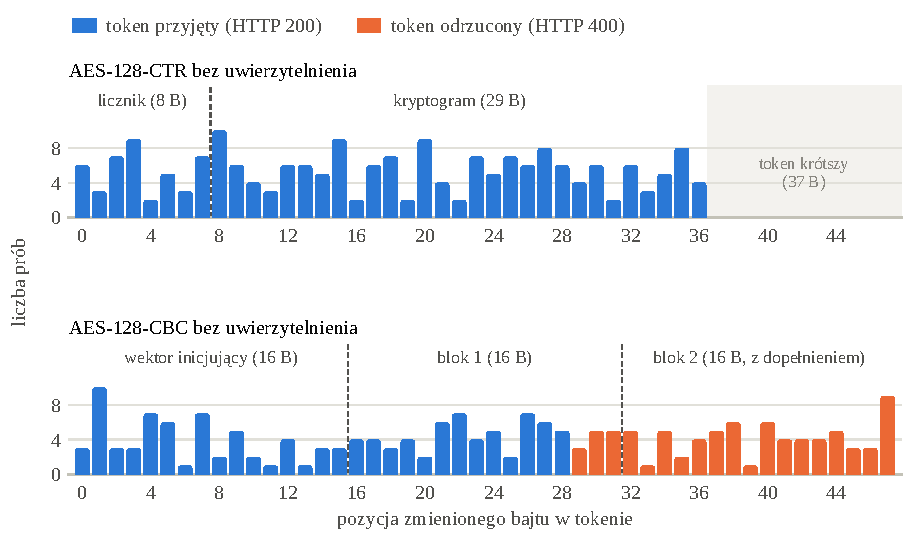
\includegraphics[width=\textwidth]{rysunki/r4-pozycje.pdf}
\caption{Wynik serii losowej w~zależności od pozycji zmienionego bajtu tokenu}
\label{rys:pozycje}
\end{figure}

Wyniki próby celowanej zawiera tabela~\ref{tab:celowane}. W~wariancie CTR zmiana jednego bajtu kryptogramu (pozycja 27, odpowiadająca wartości pola \kod{admin}) dała dokładnie zamierzony efekt: aplikacja odczytała \kod{admin=1}, pozostałe pola pozostały nienaruszone, a~użytkownik uzyskał dostęp do funkcji administracyjnych. W~wariancie GCM analogiczna zmiana została odrzucona.

\begin{table}[htbp]
\centering\small
\begin{tabularx}{\textwidth}{@{}l c c L c@{}}
\toprule
\textbf{Wariant} & \textbf{Pozycja bajtu} & \textbf{HTTP} & \textbf{Pola odczytane przez aplikację} & \textbf{Uprawnienia} \\
\midrule
AES-128-CTR & 27 & 200 & \kod{user=student}, \kod{admin=1}, \kod{uid=1001} & uzyskane \\
AES-128-CBC & 19 & 200 & \kod{uid=1001}; nazwa pola \kod{admin} zniekształcona, pole \kod{user} utracone & nie \\
AES-128-GCM & 31 & 403 & -- (token odrzucony) & nie \\
\bottomrule
\end{tabularx}
\caption{Próba celowana: zmiana wartości pola \kod{admin} z~0 na 1}
\label{tab:celowane}
\end{table}

% ---------------------------------------------------------------------
\section{Modyfikacja ciasteczka szyfrowanego w~trybie CBC}\label{sec:cbc}

Pomiar dla trybu CBC przeprowadzono tym samym skryptem, z~tymi samymi parametrami i~tym samym ziarnem co w~podrozdziale~\ref{sec:ctr}. Wariantem poprawionym był ponownie tryb GCM, dla którego wykonano osobną serię 200~prób.

\subsection*{Wyniki}

Wariant CBC bez uwierzytelnienia przyjął 120 z~200~zmodyfikowanych tokenów (60\%), a~każdy przyjęty token miał zmienioną treść (tabela~\ref{tab:cbc}). Odrzucone tokeny aplikacja odrzucała kodem 400, sygnalizującym błąd odczytu ciasteczka. Wariant GCM ponownie odrzucił wszystkie modyfikacje.

\begin{table}[htbp]
\centering\small
\begin{tabularx}{\textwidth}{@{}L rrrrc@{}}
\toprule
\textbf{Wariant} & \textbf{Próby} & \textbf{Przyjęte} & \textbf{Odsetek} & \textbf{Zmieniona treść} & \textbf{Kod odrzucenia} \\
\midrule
AES-128-CBC bez uwierzytelnienia & 200 & 120 & 60\% & 120 & 400 \\
AES-128-GCM                      & 200 &   0 &  0\% &   0 & 403 \\
\bottomrule
\end{tabularx}
\caption{Seria losowa modyfikacji ciasteczka -- szyfr blokowy}
\label{tab:cbc}
\end{table}

W~odróżnieniu od trybu CTR wynik zależał od miejsca modyfikacji (dolna część rysunku~\ref{rys:pozycje}). Wszystkie modyfikacje wektora inicjującego zostały przyjęte, modyfikacje pierwszego bloku kryptogramu -- prawie wszystkie, a~modyfikacje drugiego bloku -- żadna. Odrzucenia w~pierwszym bloku wystąpiły wyłącznie na pozycjach 29--31. Rozkład ten można przewidzieć na podstawie budowy tokenu (tabela~\ref{tab:tokeny}):
\begin{itemize}
  \item zmiana wektora inicjującego zmienia jeden bajt pierwszego bloku tekstu jawnego i~nie dotyka dopełnienia, więc token zawsze zostaje przyjęty;
  \item zmiana pierwszego bloku kryptogramu zniekształca cały pierwszy blok tekstu jawnego i~zmienia jeden bajt drugiego bloku na tej samej pozycji; token zostaje odrzucony tylko wtedy, gdy zmiana trafi w~jeden z~3~bajtów dopełnienia (pozycje 29--31), co daje oczekiwany odsetek przyjęć $13/16 = 81{,}25\%$;
  \item zmiana drugiego bloku kryptogramu zniekształca cały ostatni blok tekstu jawnego razem z~dopełnieniem; token zostanie przyjęty tylko wtedy, gdy losowy wynik przypadkiem utworzy poprawne dopełnienie, czyli z~prawdopodobieństwem około $1/256$.
\end{itemize}

Porównanie wartości zmierzonych z~oczekiwanymi zawiera tabela~\ref{tab:cbc-obszary} i~rysunek~\ref{rys:cbc-obszary}. Oczekiwany odsetek dla całej serii, ważony liczbą prób w~poszczególnych obszarach, wynosi 59,9\%, a~zmierzony 60,0\%. Zgodność ta potwierdza, że o~przyjęciu zmodyfikowanego tokenu decydowała wyłącznie poprawność dopełnienia, a~sama aplikacja nie wykrywała modyfikacji treści.

\begin{table}[htbp]
\centering\small
\begin{tabular}{@{}llrrrr@{}}
\toprule
\textbf{Obszar tokenu} & \textbf{Pozycje} & \textbf{Próby} & \textbf{Przyjęte} & \textbf{Odsetek} & \textbf{Oczekiwany} \\
\midrule
wektor inicjujący        & 0--15  &  61 &  61 & 100,0\% & 100,0\% \\
pierwszy blok kryptogramu & 16--31 &  72 &  59 &  81,9\% &  81,25\% \\
drugi blok kryptogramu    & 32--47 &  67 &   0 &   0,0\% &  $\approx 0{,}4\%$ \\
\midrule
\textbf{Razem}           & 0--47  & 200 & 120 &  60,0\% &  59,9\% \\
\bottomrule
\end{tabular}
\caption{Wariant CBC: odsetek przyjętych modyfikacji według obszaru tokenu}
\label{tab:cbc-obszary}
\end{table}

\begin{figure}[htbp]
\centering
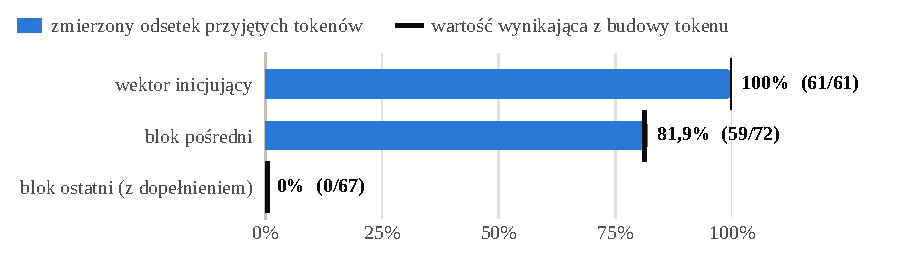
\includegraphics[width=\textwidth]{rysunki/r4-cbc-obszary.pdf}
\caption{Wariant CBC: zmierzony odsetek przyjętych tokenów na tle wartości wynikającej z~budowy tokenu}
\label{rys:cbc-obszary}
\end{figure}

Próba celowana w~trybie CBC nie dała napastnikowi uprawnień (tabela~\ref{tab:celowane}). Wartość pola \kod{admin} znajduje się w~drugim bloku tekstu jawnego (bajt 19), więc jej zmiana wymaga modyfikacji pierwszego bloku kryptogramu, która zniekształca cały pierwszy blok tekstu jawnego -- \kod{user=student;adm}. Aplikacja odczytała wprawdzie wartość~1, ale pod zniekształconą nazwą pola, przez co nie rozpoznała jej jako pola \kod{admin}. O~niepowodzeniu zdecydował więc układ danych w~blokach, a~nie właściwość trybu: gdyby modyfikowane pole leżało w~pierwszym bloku, zmianę można by przeprowadzić przez wektor inicjujący, którego modyfikacje były przyjmowane w~100\% przypadków i~nie zniekształcały pozostałych danych.

Pomiar ujawnił też dodatkową słabość wariantu podatnego: aplikacja odpowiadała innym kodem na błąd dopełnienia (400) niż na pozostałe błędy weryfikacji. Rozróżnialne komunikaty o~błędzie dopełnienia ujawniają informację o~poprawności odszyfrowanych danych i~w~przeszłości stanowiły podstawę skutecznych ataków na tryb CBC~\cite{boneh2023}. Niezależnie od zmiany trybu szyfrowania zaleca się więc zwracanie jednakowej odpowiedzi dla wszystkich błędów odczytu ciasteczka.

% ---------------------------------------------------------------------
\section{Weryfikacja podpisu żądań: SHA-256(sekret~$\|$~wiadomość) a~HMAC}\label{sec:lenext}

Aplikacja testowa uwierzytelnia żądania API podpisem dołączanym do treści żądania. W~wariancie podatnym podpis to skrót SHA-256 z~połączenia sekretu i~wiadomości, a~w~wariancie poprawionym -- kod HMAC-SHA-256 (tabela~\ref{tab:aplikacja}). Oba warianty korzystają z~tego samego 16-bajtowego sekretu, losowanego przy starcie aplikacji.

\subsection*{Przebieg pomiaru}

Skrypt \kod{r4-pomiar-integralnosci.py} pobierał z~aplikacji poprawnie podpisane żądanie przelewu, a~następnie wysyłał do każdego wariantu pięć jego odmian: żądanie nienaruszone, żądanie ze zmienioną wartością pola, żądanie z~doklejonym na końcu dodatkowym polem (bez zmiany podpisu), żądanie ze zmienionym jednym znakiem podpisu oraz żądanie z~podpisem losowym. Dla każdej odmiany zapisywano kod odpowiedzi HTTP.

\subsection*{Wyniki}

Wyniki zestawiono w~tabeli~\ref{tab:podpis}. Oba warianty przyjęły wyłącznie żądanie nienaruszone, a~wszystkie cztery naruszenia pary (wiadomość, podpis) odrzuciły kodem 403. Weryfikacja podpisu jest więc w~obu wariantach zaimplementowana poprawnie i~test czarnoskrzynkowy nie odróżnia od siebie obu konstrukcji.

\begin{table}[htbp]
\centering\small
\begin{tabular}{@{}lcc@{}}
\toprule
\textbf{Przypadek} & \textbf{SHA-256(sekret~$\|$~wiadomość)} & \textbf{HMAC-SHA-256} \\
\midrule
żądanie nienaruszone                    & 200 -- przyjęte   & 200 -- przyjęte \\
zmieniona wartość pola                  & 403 -- odrzucone  & 403 -- odrzucone \\
doklejone pole, podpis bez zmian        & 403 -- odrzucone  & 403 -- odrzucone \\
zmieniony jeden znak podpisu            & 403 -- odrzucone  & 403 -- odrzucone \\
podpis losowy                           & 403 -- odrzucone  & 403 -- odrzucone \\
\bottomrule
\end{tabular}
\caption{Reakcja aplikacji na naruszenie pary (wiadomość, podpis)}
\label{tab:podpis}
\end{table}

Różnica między wariantami wynika z~budowy funkcji skrótu, a~nie z~implementacji weryfikacji. Funkcja SHA-256 ma konstrukcję Merkle'a--Damgårda, w~której wynik jest stanem wewnętrznym po przetworzeniu ostatniego bloku danych. Znając podpis $\mathrm{SHA\text{-}256}(s \| m)$ oraz długość sekretu, można więc obliczyć poprawny podpis dla wiadomości przedłużonej o~dopełnienie i~dowolny sufiks, nie znając sekretu (atak przedłużenia, ang. \ang{length extension}). Konstrukcja HMAC przetwarza wynik wewnętrznego skrótu drugi raz, z~innym kluczem, i~tej własności nie ma (podrozdział~\ref{sec:skroty})~\cite{boneh2023}. Przypadek z~doklejonym polem odrzucono w~obu wariantach, ponieważ nie zmieniono podpisu; pomiar nie obejmował obliczania podpisu dla wiadomości przedłużonej. Podatność wariantu z~konstrukcją $\mathrm{SHA\text{-}256}(s \| m)$ wynika więc z~analizy konstrukcji, a~pomiar potwierdza jedynie, że pozostałe elementy weryfikacji działają w~obu wariantach tak samo.

% ---------------------------------------------------------------------
\section{Podsumowanie wyników}\label{sec:ataki-podsum}

Odsetek przyjętych zmodyfikowanych ciasteczek w~trzech badanych trybach szyfrowania zestawiono na rysunku~\ref{rys:odsetek}, a~wyniki wszystkich eksperymentów rozdziału -- w~tabeli~\ref{tab:r4-podsum}.

\begin{figure}[htbp]
\centering
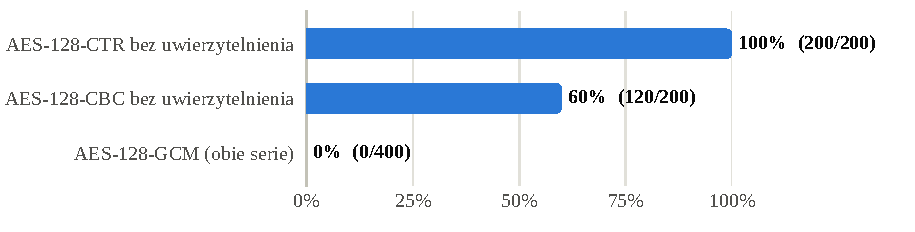
\includegraphics[width=\textwidth]{rysunki/r4-odsetek.pdf}
\caption{Odsetek przyjętych zmodyfikowanych ciasteczek w~seriach losowych}
\label{rys:odsetek}
\end{figure}

\begin{table}[htbp]
\centering\small
\begin{tabularx}{\textwidth}{@{}>{\raggedright\arraybackslash}p{2.6cm} L L@{}}
\toprule
\textbf{Mechanizm} & \textbf{Wariant podatny -- wynik} & \textbf{Wariant poprawiony -- wynik} \\
\midrule
podszycie w~ARP & -- & inspektor \kod{arp\_spoof}: 3 z~3 ramek wykryte (6~alarmów), 0~alarmów dla ogłoszeń poprawnych \\
negocjacja TLS & OpenSSL 1.0.2u: 4 z~5 wersji, w~tym SSLv3; SCSV działa tylko dla klienta, który go wyśle & nginx: wyłącznie TLS~1.2 i~1.3 z~zestawami AEAD; SCSV działa \\
ciasteczko, szyfr strumieniowy & AES-CTR: 100\% modyfikacji przyjętych, uprawnienia administratora uzyskane & AES-GCM: 0\% przyjętych \\
ciasteczko, szyfr blokowy & AES-CBC: 60\% przyjętych, zgodnie z~modelem (59,9\%); próba celowana nieudana z~powodu układu danych & AES-GCM: 0\% przyjętych \\
podpis żądania & SHA-256(sekret~$\|$~wiadomość): naruszenia odrzucone, konstrukcja podatna na atak przedłużenia & HMAC-SHA-256: naruszenia odrzucone, konstrukcja odporna \\
\bottomrule
\end{tabularx}
\caption{Zestawienie wyników rozdziału~\ref{ch:ataki}}
\label{tab:r4-podsum}
\end{table}

Z~przeprowadzonych eksperymentów wynikają następujące wnioski:
\begin{enumerate}
  \item \textbf{Poufność nie zapewnia integralności.} Oba tryby bez uwierzytelnienia przyjmowały zmodyfikowane dane, mimo że napastnik nie znał klucza. Tryb GCM odrzucił wszystkie 400~modyfikacji w~obu seriach.
  \item \textbf{Podatność zależy od budowy trybu.} W~trybie CTR każda zmiana została przyjęta, a~zmiana celowana dała dokładnie zamierzony efekt. W~trybie CBC skutek zależał od położenia zmiany, a~zmierzony rozkład zgadzał się z~wartością wynikającą z~budowy tokenu z~dokładnością do 0,1~punktu procentowego.
  \item \textbf{Ochrona przed obniżeniem wersji musi być po stronie serwera.} Mechanizm SCSV działa tylko wtedy, gdy klient sam zasygnalizuje ponowienie połączenia. Pewną ochronę daje dopiero wyłączenie wersji starszych niż TLS~1.2.
  \item \textbf{Próby ataku pozostawiają ślad w~ruchu sieciowym.} Zarówno podszycie w~ARP, jak i~zestawienie sesji z~przestarzałymi parametrami są widoczne dla czujnika. Na tej obserwacji oparto warstwę detekcji sieciowej opisaną w~rozdziale~\ref{ch:obrona}.
\end{enumerate}
